\chapter{Fachkonzept}
\section{Anforderungen}

%Kurze Anforderungsanalyse und USE-Case beschreiben
Abbildung \ref{fig:abb1} zeigt ein vereinfachtes Use Case Diagramm für den Spieler. Diese Anforderungen müssen in der Benutzeroberfläche und im tatsächlichen Fachkonzept umgesetzt werden. \\
Um ein neues Spiel zu spielen, muss der Spieler ein Spiel starten können. Dies beinhaltet, dass ein Spielbrett erzeugt, ein Segment gewählt werden kann und in diesem Segment eine Standarduhr mit den ersten Attributen freigeschaltet wird. Je nach Segment werden verschiedene Kosten vom Kapital abgezogen um somit das Verhältnis von Billig zu Teuer zu gewährleisten. \\
Währen dem Spiel kann der Spieler verschiedenes in seinem Unternehmen machen, wie zum Beispiel die Produktion erweitern, Attribute entwickeln, Uhren produzieren und verkaufen. Weitere Aufgaben können aus dem Use Case abgelesen werden. Sobald ein Spieler seine Uhr verbessert / produziert oder die Absatzmenge angegeben hat, wird die Runde beendet. In diesem Schritt werden die Spielerdaten gespeichert und somit auch die neue Konfiguration der Uhr berechnet. Anschließend ist der nächste Spieler an der Reihe. Sollte eine Runde von allen Spielern beendet worden sein ist die erste Periode zu Ende und die Marktsimmulation wird gestartet.

\begin{figure}[!h]
	\centering
	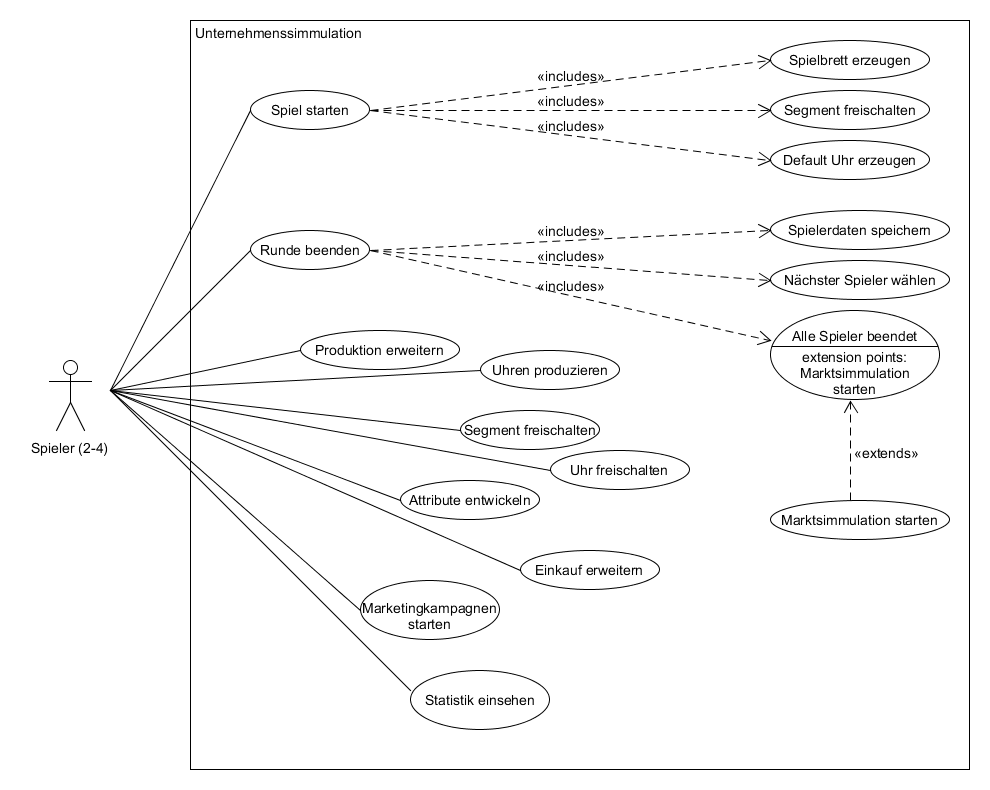
\includegraphics[scale=0.4]{img/UseCase.png} 
	\caption{Vereinfachtes Use Case} \label{fig:abb1}
\end{figure}

\newpage
\section{Klassen}
Im folgenden Abschnitt werden die einzelnen Klassen mit den wichtigsten Methoden kurz erläutert. Ein komplettes Klassendiagramm ist in Abbildung \ref{fig:abb27} dargestellt. Der Markt wird im Kapitel \ref{KapitelMarkt} genauer beschrieben.

\subsection{Spielbrett}
Das Spielbrett managed den kompletten Spielablauf. Im ersten Schritt wird ein Spielbrett mit der Anzahl der Runden, dem Marktvolumen und dem Einflussbereich für den Markt erzeugt. Anschließend kann der erste Spieler sein Unternehmen leiten. Sobald er die Runde beendet, wird der nächste Spieler ausgewählt bis alle Spieler die Periode abgeschlossen haben. Mit abschließen der Periode wird die Martsimmulation gestartet. Genaueres im Kapitel \ref{KapitelMarkt}. \\
Nachdem alle Runden gespielt und die Marktsimmulation am Ende noch einmal durchgelaufen ist, wird der Sieger ermittelt. Die Methode der Gewinnermittlung ist im folgenden aufgezeigt: \\

\lstset{language=Java} 
\begin{lstlisting} [caption={Gewinnermittlung},captionpos=b]
private void gewinnermittlung() {
	this.sieger = new int[spieler.length];
	double kapi[] = new double[spieler.length];
	
	// Kapital in extra array speichern
	for(int i = 0; i < spieler.length; i++)
	kapi[i] = spieler[i].getKapital();
	
	// Kapitel nach der groesse sortieren und umdrehen		
	Arrays.sort(kapi);
	double temp[] = new double[kapi.length];
	int t = kapi.length-1;
	for(int i = 0; i < kapi.length; i++)
	{
		temp[t] = kapi[i];
		t--;
	}
	kapi = temp;
	
	// Kapital den Siegern zuordnen und in siegerarray speichern
	for(int i = 0; i < spieler.length; i++) {
	for(int j = 0; j < kapi.length; j++)
		if(kapi[i] == spieler[j].getKapital()) {
		sieger[i] = j;
		break;
		}
	}
}
\end{lstlisting}

Nachdem der Gewinner ermittelt und auf der Benutzeroberfläche angezeigt wurde, kann ein neues Spiel gestartet werden und die Simulation startet von vorn.

\newpage
\subsection{Unternehmen}
Abbildung \ref{fig:abb2} zeigt zunächst ein Klassendiagramm, um einen groben Überblick zu erhalten. Üblicherweise sind die Attribute und Methoden in einem Klassendiagramm untereinander, jedoch aus Platzgründen wurde es hier nebeneinander dargestellt.

\begin{figure} [h]
	\centering
	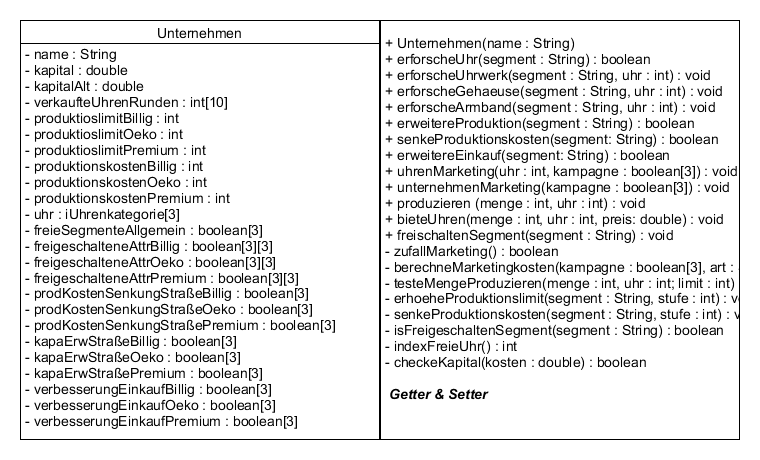
\includegraphics[scale=0.6]{img/Unternehmen.png} 	
	\caption{Klassendiagramm Unternehmen} \label{fig:abb2}
\end{figure}

Im Unternehmen sind alle wichtigen Attribute gespeichert, die zu einem Unternehmen / Spieler gehören. Da der Spieler das Unternehmen leitet, wird im folgenden das Unternehmen benannt. \\

Das Interface iUhrenkategorie bietet die Methodensignaturen für die verschiedenen Uhren an und wird somit als Schnittstelle verwendet. Damit das Unternehmen alle Uhren in einem Array vereinen kann, wird Polymorphie angewandt. Im folgenden Codeabschnitt wird gezeigt, wie Polymorphie in Java verwendet wird. \\

\lstset{language=Java} 
\begin{lstlisting} [caption={Interface iUHrenkategorie},captionpos=b]
	private iUhrenkategorie uhr[] = new iUhrenkategorie[3];
	
	uhr[0] = new BilligUhr();
\end{lstlisting}

Das Attribut \textit{uhr} wird als iUhrenkategorie-Array mit der Größe drei erzeugt. Anschließend wird im ersten Feld eine BilligUhr erzeugt. Durch Polymorphy wird eine Referenzvariable vom Typ iUhrenkategorie erstellt. Somit können die verschiedenen Uhrenkategorien in einem Array erstellt und im Anschluss verwendet werden. 

Im folgenden Abschnitt werden die wichtigsten Methoden der Klasse erläutert. Viele der Methoden sind durch ein switch-case in die Segmente unterteilt. Da sich der Codeteil nur um die Attributnamen verändert, wurden diese Codestücke durch [...] ersetzt.

\subsubsection{Uhr erforschen}
Das erforschen der Uhr ist einer der wichtigsten Methoden im Unternehmen. Sobald das Spiel gestartet und der Spieler ein Segment gewählt hat, wird eine Standarduhr in dem Segment erforscht. Alle weiteren Uhren können während dem Spiel erforscht werden, sofern genügend Kapital vorhanden ist. 

\lstset{language=Java} 
\begin{lstlisting}[caption={Neue Uhr erforschen},captionpos=b]
public boolean erforscheUhr(String segment) {
	boolean result = false;
	// Test auf naechste Freie Uhr
	int index = indexFreieUhr();
	
	// Wenn alle Uhren entwickelt oder nicht genug Kohle-> false zurueckgeben;
	if(index != -1 ) {
		// Checken ob Segment bereits freigeschalten
		if(isFreigeschaltenSegment(segment)) {
			switch(segment) {
				case "Billig":
					if(checkeKapital(Info.getKostenUhrBillig())) {
						this.uhr[index] = new BilligUhr();
						result = true;
					}
					else
						System.out.println("Nicht genug Kohle!");
					break;
				case "Premium":
					[...]
				case "Oeko":
					[...]
				default:
					System.out.println("Falsches Segment");
					break;
			}
		}
		else {
			System.out.println("Segment noch nicht freigeschalten");
		}
	}
	else {
		System.out.println("Es kann keine weitere Uhr erforscht werden!");
	}
	return result;
}
\end{lstlisting}

Zunächst wird überprüft, ob noch eine weitere Uhr erforscht werden kann. Jedes Unternehmen kann 3 Uhren entwickeln bzw. erforschen. Als nächstes wird geschaut, ob das passende Segment schon erforscht wurde, in dem die Uhr erstellt werden soll. Als letzte Abfrage wird über ein switch-case das Segment gewählt und die passende Uhr am passenden Indexplatz erzeugt.

\subsubsection{Produktion erweitern}

\lstset{language=Java} 
\begin{lstlisting} [caption={Produktion erweitern},captionpos=b]
public boolean erweitereProduktion(String segment) {
	// Erweitert die Kapazitaet -> erhoeht also das Produktionslimit
	switch(segment) {
		case "Billig":
			for(int i = 0; i < 3; i++) {
				if(this.getKapaErwStrasseBillig()[i] == false) {
					if(checkeKapital(Info.getKostenProduktionBillig()[i])) {
					kapaErwStrasseBillig[i] = true;
					erhoeheProduktionslimit(segment, i);
					return true;
				}
			}
		}
		break;
		case "Premium":
			[...]
		}
		break;
		case "Oeko":
			[...]
		}
		break;
		default:
			System.out.println("Falsches Segment");
			break;
	}
	return false;
}	
\end{lstlisting}

Diese Methode wählt zunächst über ein Switch-Case das Segment aus, in dem das Produktionslimit erhöht werden soll. Anschließend wird überprüft, ob genügend Kapital vorhanden ist um die Produktion zu erweitern. Diese Kosten werden aus der Klasse \textit{Info.java} ausgelesen. Wenn genug Kapital vorhanden ist, werden die Kosten abgezogen und das passende Feld im Array wird freigeschalten.

\subsubsection{Uhren produzieren}
Diese Methode ist auch ein wichtiger Bestandteil des Unternehmens. Hier werden die Uhren produziert. Als Übergabeparameter werden die Menge und die Uhr übergeben. 

Zunächst wird überprüft, ob diese Uhr überhaupt existiert und somit wird ein falscher Aufruf abgefangen. Als nächstes werden die Selbstkosten der Uhr berechnet und gegebenenfalls mit einem Faktor Einkauf verrechnet. Der Faktor Einkauf wird dann gesetzt, wenn eine Erweiterung im Einkauf stattgefunden hat. Solange dieser nicht erweitert wurde, bleibt der Faktor 0.

Als nächstes wird mit der privaten Methode \textit{testeMengeProduzieren} getestet, ob die gewünschte Menge produziert werden kann. Sollte nicht genügend Kapital vorhanden sein, wird die Menge berechnet, die mit dem letzten Kapital noch Produziert werden kann. Im letzten Schritt wird der neue Bestand gesetzt und das Kapital um die Kosten verringert.

\lstset{language=Java} 
\begin{lstlisting} [caption={Gewünschte Menge produzieren},captionpos=b]
public void produzieren(int menge, int uhr) {
	if(this.uhr[uhr] != null) {
		int m = 0;
		double s = this.uhr[uhr].berechneSelbstkosten();
		double f = 0;
		// Segment abfragen
		switch(this.uhr[uhr].getSegment()) {
			case "Billig":
				f = sucheEinkaufsfaktor("Billig");
				if(f != 0)
					s *= f;
				m = testeMengeProduzieren( menge, uhr , this.getProduktionslimitBillig(), s);
				if(m != -1) {
					this.setKapital( this.getKapital() - (m * s) );
					this.uhr[uhr].setBestand(this.getBestandUhr(uhr) + m);
				}
				break;
			case "Oeko":
				...
			case "Premium":
				...
		}
	}
}

private int testeMengeProduzieren(int menge, int uhr, int limit, double prodKostenStueck) {
	int m = -1;
	// Produktionslimit testen
	if( (menge + this.getBestandUhr(uhr) ) > limit)
		menge = limit;
		// Berechnen wie viele mit vorhandenem Kapital produziert werden koennen
		for(int i = menge; i > 0; i --) {
			double prodKosten = i * prodKostenStueck;
			if(prodKosten <= this.getKapital()) {
			m = i;
			break;
		}
	}
	return m;
}
\end{lstlisting}

\subsubsection{Segment freischalten}
Diese Methode schaltet ein neues Segment frei. Als Übergabeparameter wird das Segment mitgegeben, welches freigeschaltet werden soll. Wenn genügend Kapital vorhanden ist, wird das Segment freigeschaltet.

\lstset{language=Java} 
\begin{lstlisting} [caption={Weiteres Segment freischalten},captionpos=b]
public void freischaltenSegment(String segment) {
	switch(segment) {
		case "Billig":
		if(checkeKapital(Info.getKostenSegmentBillig())) {
			if(this.freieSegmenteAllgemein[0] == false)
				this.freieSegmenteAllgemein[0] = true;
			}
		break;
		case "Oeko":
			[...]
		break;
		case "Premium":
			[...]
		break;
	}
}
\end{lstlisting}

\subsubsection{Attribute entwickeln}
In diesem Abschnitt werden die Attribute Uhrwerk, Gehäuse und Armband entwickelt. Da die Methoden ähnlich sind, wird hier als Codebeispiel nur das Uhrwerk angegeben. Der Übergabeparameter ist das Segment und der Index, welche Erweiterung freigeschaltet werden soll. Nachdem das Kapital ausreichend ist, wird das Attribut entwickelt. Das Entwickeln wird in der Klasse Uhrmodell ausgelagert, da dies für alle Uhren identisch ist und somit kein Wiederholender Code geschrieben wird.

\lstset{language=Java}
\begin{lstlisting} [caption={Weiteres Uhrwerk erforschen},captionpos=b]
public void erforscheUhrwerk(String segment, int index) {
	double kosten = 0;
		switch (segment) {
		case "Billig":
			kosten = Info.getKostenUhrwerkBillig()[index];
			if(checkeKapital(kosten))
			freigeschalteneAttrBillig = Uhrmodell.entwickleUhrwerk(freigeschalteneAttrBillig, 2);
		break;
		case "Oeko":
			[...]				
		break;
		case "Premium":
			[...]
		break;
	}	
}
\end{lstlisting}

\subsubsection{Einkauf erweitern}
In dieser Methode wird der Einkauf erweitert und somit die Anschaffungskosten der Uhr geringer. Sollte genügend Kapital vorhanden sein, so wird ein Flag gesetzt, welches in der Methode \textit{produzieren} abgefragt und mit den Selbstkosten verrechnet wird. Als Übergabeparameter wird das Segment übergeben.

\lstset{language=Java}
\begin{lstlisting}[caption={Einkauf erweitern},captionpos=b]
public boolean erweitereEinkauf(String segment) {
	switch(segment) {
		case "Billig":
			for(int i = 0; i < 3; i++) {
				if(verbesserungEinkaufBillig[i] == false) {
					if(checkeKapital(Info.getKostenEinkaufBillig()[i])) {
						verbesserungEinkaufBillig[i] = true;
						return true;
					}
				}
			}
			break;
		case "Premium":
			[...]
		break;
		case "Oeko":
		for(int i = 0; i < 3; i++) {
			[...]
		break;
		default:
			System.out.println("Falsches Segment");
		break;
	}
	return false;
}
\end{lstlisting}

\subsubsection{Marketingkampagnen starten}
Als Marketingkampagnen sind zwei verschiedene Arten vorgesehen. Als erstes ein Marketing speziell für die Uhr und ein Unternehmensmarketing. Das spezielle Marketing der Uhr verändert nur den Score der einen Uhr, bei der eine Kampagne gestartet werden soll. Im Unternehmensmarketing hingegen wirkt sich die Kampagne auf alle Uhren des Unternehmens aus.

Bei beiden Varianten wird eine Zufallskomponente eingebaut, die über den Erfolg bzw. Misserfolg einer Marketingkampagne entscheidet. Diese Zufallskomponente erstellt eine zufällige Zahl zwischen 0 und 1. Sollte der Wert zwischen 0,4 und 0,6 liegen, scheitert die Marketingkampagne.

\lstset{language=Java}
\begin{lstlisting} [caption={Marketingkampagne starten},captionpos=b]
public void uhrenMarketing(int uhr, boolean[] kampagne) {	
	// Kosten der Kampagnen berechnen
	double kostenMarketing = berechneMarketingkosten(kampagne, "Uhr");
	
	// Suche den Index
	int boostIndex = -1;
		for(int i = 0; i < 3; i++) {
		if(kampagne[i] == true)
		boostIndex = i;
	}
	
	// Nur wenn Kapital ausreichend ist
	if(checkeKapital(kostenMarketing)){
		// Nur Boosten, wenn Zufallszahl nicht zugeschlagen hat
		if(boostIndex != -1 && zufallMarketing()) {
			this.uhr[uhr].setMarketingboost(this.uhr[uhr].getMarketingboost() + Info.getScoreMarketingkampagne()[boostIndex]);
		} else {
			this.uhr[uhr].setMarketingboost(this.uhr[uhr].getMarketingboost());				
		}
	}

}

public void unternehmenMarketing(boolean[] kampagne) {
	// Kosten der Kampagnen berechnen
	double kostenMarketing = berechneMarketingkosten(kampagne, "Unternehmen");
	// Suche den Index
	int boostIndex = -1;
		for(int i = 0; i < 3; i++) {
		if(kampagne[i] == true)
		boostIndex = i;
	}
	
	// Nur wenn Kapital ausreichend ist 
	if(checkeKapital(kostenMarketing)) {
		if(boostIndex != -1 && zufallMarketing()) {
		// Marketingbosst auf alle Uhren anrechnen wenn Zufallszahl nicht zugeschlagen hat
		for(int i = 0; i < 3; i++) {
			if(this.uhr[i] != null)
			this.uhr[i].setMarketingboost(this.uhr[i].getMarketingboost() + Info.getScoreMarketingkampagne()[boostIndex]);
			}
		} else {
			for(int i = 0; i < 3; i++) {
				if(this.uhr[i] != null)
				this.uhr[i].setMarketingboost(this.uhr[i].getMarketingboost());
			}
		}
	}
}

// Zufall einbauen
private boolean zufallMarketing() {
	// Zufallszahl zwischen 0 und 1
	Random rand = new Random();
	double z = rand.nextDouble();
	// zwischen 0.4 und 0.6 (incl)
	if(z >= 0.4 && z <= 0.6)
		return false;
	return true;
}
\end{lstlisting}

\subsubsection{Kapital überprüfen}
Diese Methode ist zwar klein, aber fein. Sie bestimmt bei fast allen Methoden ob das Kapital ausreichend für die benötigten Kosten sind. Ohne diese Methode könnte das Unternehmen alles entwickeln und hätte sozusagen unendliches Geld zur Verfügung.
Sollte genügend Kapital vorhanden sein, dann werden die Kosten vom Kapital abgezogen und es wird \textit{true} zurückgegeben.

\lstset{language=Java}
\begin{lstlisting} [caption={Überprüfung vorhandenes Kapital},captionpos=b]
private boolean checkeKapital(double kosten) {
	if( (this.kapital - kosten) >= 0) {
		this.kapital -= kosten;
		return true;
	}
	else
		return false;
}
\end{lstlisting}

\subsection{Uhren}
Hierunter zählen die Klassen BilligUhr, OekoUhr und PremiumUhr. Alle Klassen implementieren das Interface iUhrenkategorie und müssen alle Methoden des Interfaces implementieren. Das Unternehmen hat Zugriff auf alle implementierten Methoden, die im Interface erstellt wurden, durch die Polymorphie. 

Die Uhren-Klassen dienen nur als Datenverwaltung, damit die Konfiguration der Uhren im Unternehmen gespeichert werden können. Die wichtigsten Methoden sind: 

\lstset{language=Java}
\begin{lstlisting} [caption={Selbstkosten/Marktwert berechnen},captionpos=b]
public double berechneSelbstkosten() {
	return( Info.getSelbstkostenArmbandBillig()[this.getArmband()] + Info.getSelbstkostenGehaeuseBillig()[this.getGehaeuse()] 
	+ Info.getSelbstkostenUhrwerkBillig()[this.getUhrwerk()] );
}

public double berechneMarktwert() {
	this.setMarktwert( this.getSelbstkosten() * (1 + ( Info.getScoreArmbandBillig()[this.getArmband()] + Info.getScoreGehaeuseBillig()[this.getGehaeuse()] + 
	Info.getScoreUhrwerkBillig()[this.getUhrwerk()])) ); 
	return this.getMarktwert();
}
\end{lstlisting}

Beide Methoden sind mit \textit{@Override} versehen. Dies zeigt, dass die Methode vom Interface überschrieben werden müssen, also ein Methodenbody eingefügt werden muss. Um die Selbstkosten zu berechnen, wird die Konfiguration der Uhr multipliziert mit den Kosten, die für diese Konfiguration stehen. Diese Kosten werden aus der Klasse \textit{Info.java} ausgelesen.\\

Der Merktwert der Uhren wird berechnet aus den Selbstkosten multipliziert mit (1 + Score der Attribute). Je hochwertiger die Konfiguration der Uhr ist, desto höher ist der Score und somit steigt auch der Marktwert der Uhr an.

\subsection{Interface iUhrenkategorie}
Das Interface stellt alle Methoden für die Uhren zur Verfügung. An dieser Stelle nur das Klassendiagramm des Interfaces in Abbilung \ref{fig:abb3}. Die wichtigsten Methoden werden im Abschnitt Unternehmen erläutert.

\begin{figure}[!h]
	\centering
	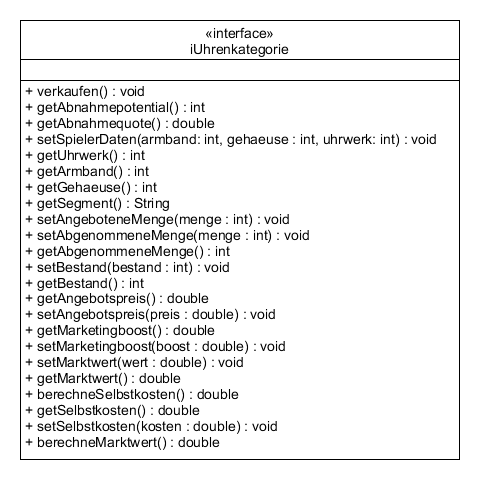
\includegraphics[scale=0.7]{img/iUhrenkategorie.png} 
	\caption{Klassendiagramm iUhrenkategorie} \label{fig:abb3}
\end{figure}

\subsection{Uhrmodell}
Die Klasse Uhrmodell wird als statische Klasse implementiert und dient dazu, gleiche Methoden der Uhren auszulagern. Die Klasse besteht aus 3 Methoden: 

\lstset{language=Java}
\begin{lstlisting} [caption={Weiteres Merkmal entwickeln},captionpos=b]
public static boolean[][] entwickleUhrwerk(boolean[][] uhrwerk, int index) {
	for(int i = 0; i < 3; i++) {
		if(uhrwerk[index][i] == false) {
			uhrwerk[index][i] = true;
			break;
		}
	}
	return uhrwerk;
}

public static boolean[][] entwickleArmband(boolean[][] armband, int index) {
	for(int i = 0; i < 3; i++) {
		if(armband[index][i] == false) {
			armband[index][i] = true;
			break;
		}
	}
	return armband;
}

public static boolean[][] entwickleGehaeuse(boolean[][] gehaeuse, int index) {
	for(int i = 0; i < 3; i++) {
		if(gehaeuse[index][i] == false) {
			gehaeuse[index][i] = true;
			break;
		}
	}
	return gehaeuse;
}	
\end{lstlisting}

Diese statischen Methoden erweitern das Uhrwerk, das Armband und das Gehäuse der Uhr. Als Übergabeparameter wird das gesamte Array und der feste Index übergeben. Anschließend wird das nächste Attribut freigeschaltet und das erweiterte Array zurückgegeben. Durch die statischen Methoden muss von dieser Klasse keine Instanz erstellt werden und die Methodenaufrufe erfolgen über den Klassennamen.

\subsection{Info}
Die Info.java dient ausschließlich der Informationsverwaltung. In dieser statischen Klasse werden die Attributnamen, die Kosten und die verschiedenen Faktoren bereitgestellt. Da dies eine statische Klasse ist, wird keine Instanz verwendet, sondern die Methoden können über den Klassennamen aufgerufen werden. \\
Beispiel:

\lstset{language=Java}
\begin{lstlisting} [caption={Beispielaufruf aus Info.java},captionpos=b]
	double kosten = Info.getSelbstkostenGeaeuseBillig()[0];
\end{lstlisting}